\documentclass[12pt]{article}
\usepackage[margin=1in]{geometry}                % See geometry.pdf to learn the layout options. There are lots.
\geometry{letterpaper}                   
\usepackage{graphicx}
\usepackage{amssymb}
\usepackage{epstopdf}
\DeclareGraphicsRule{.tif}{png}{.png}{`convert #1 `dirname #1`/`basename #1 .tif`.png}

\raggedright % So not straight on both sides
\setlength{\parindent}{0.5in} % So indent paragraphs
\usepackage{indentfirst} % So indent first paragraph after a heading
\usepackage{titlesec}
\usepackage{authblk}
\titleformat{\section}[block]{\normalsize \bfseries \filcenter}{}{1em}{}
\titleformat{\subsection}[block]{\normalsize \bfseries}{}{1em}{}
\titleformat{\subsubsection}[runin]{\bfseries}{}{}{}[]
\titlespacing{\subsubsection}{\parindent}{*2}{\wordsep}
\setcounter{secnumdepth}{0}
\usepackage{setspace}
\usepackage{apacite}
\usepackage{amsmath}
\usepackage{color} % So can change text colour, helpful for editting
\usepackage[usenames,dvipsnames,svgnames,table]{xcolor}
\usepackage{graphicx} % So can add pictures
\usepackage[labelfont=it, labelsep=period]{caption} % So can change figure 1 to italics
\usepackage{enumitem} % To format lists ok
\usepackage{rotating}

\usepackage{fancyhdr} % To add headers
\fancyhf{}
\fancyhead[LO]{\iffloatpage{}{\nouppercase\rightmark}}
\fancyhead[RE]{\iffloatpage{}{\nouppercase\leftmark}}
\fancyhead[RO,LE]{\iffloatpage{}{\thepage}}
\renewcommand{\headrulewidth}{\iffloatpage{0pt}{0.4pt}}
\renewcommand{\footrulewidth}{0pt}
\pagestyle{fancy}

\usepackage{lastpage}
\lhead[NS01]{NS01}


\title{NS01: Binary choice vs. strength-of-preference}
\author{C. E. R. Edmunds}
\date{}
\begin{document}

\maketitle

% \newpage
% \begin{abstract}
% \end{abstract}
\doublespacing

\section{Notes}
People to email results: najmi.husaini@warwick.ac.uk

\section{Rationale}

EQ4D

average number of fixations per picture?

We are interested in the effects of attention (as measured by time spent looking at an object using eye-tracking) and value (as elicited from the subjects directly via ratings) when determining choices between two objects (such as between two bags of chips, or two pictures of nature, or between two fruits). In previous experiments, we have found that choice is predicted by an interaction of attention and value: people attend to objects they like more and are more likely to choose them. However, in other experiments there are only additively separable effects of attention and value on choice: people are more likely to pick the option they value more and/or they are more likely to choose the option they attend to more, but that these effects do not interact (i.e. looking more does not have a bigger effect when the value difference is bigger). 
 
The current experiment will attempt to identify which properties lead to the interactive vs. additive effect of attention and value. Here, we will compare simple binary choice between two pictures (Would you prefer Picture A or Picture B on your wall?) with a strength of preference comparison (By how much would you prefer Picture A over Picture B, or vice versa?). We hypothesise that the size of the interaction term will be greater in the strength-of-preference condition than in the choice condition. 

\section{Method}
\subsection{Participants}

Data was collected from $67$ participants: $2$ of these were excluded because the eye-tracker would not initially calibrate and $12$ of these were excluded due to a coding error which meant the fixation cross did not work for them. This resulted in data being collected from $53$ participants. All participants were recruited from the University of Warwick’s volunteer subject pool and paid £10 for their participation.

\subsection{Apparatus}
The participants were tested individually using an EyeLink 1000 Plus (SR Research, Osgoode, ON, Canada) eye-tracker. Monocular eye movements were recorded at 500Hz and fixations were identified by the eye tracker using velocity algorithms. The Areas of Interest were defined as a rectangle around the image position(s) on the screen. The experiment was displayed on a widescreen monitor (1920 x 1080 resolution, refresh). Participants were placed on a chin rest approximately 70cm away from the screen. Stimulus presentation was controlled by MATLAB using Psychtoolbox extensions \cite{Brainard1997, Pelli1997}.
% TODO Find refresh rate of screen

\subsection{Design}
All participants completed binary choice and strength-of-preference tasks in a counterbalanced order, followed by a final valuation task where they had to rate their overall liking for each picture on a Likert scale. 

\subsection{Stimuli and choices}
The stimuli were chosen from the International Affective Picture System \cite{Lang:2008}. The pictures were all positive in affect (average, male and female ratings between 5=neutral and 7=mildly positive) and had differences in value ratings of no more than 1.5 between male and female raters. After visual inspection, a further 7 images were removed for containing sexual images and 32 images were removed because they had a portrait aspect ratio. The 200 stimuli for each participant were randomly sampled without replacement from the 253 pictures that met these criteria. The participant's choices were generated by pairing the first stimulus with the hundred-and-first, the second with the hundred-and-second and so forth. 

\subsection{Procedure}
The experiment was displayed on a black background with white text and response scales. At the beginning of the experiment the participants were asked to provide their age and gender. Then, participants completed three tasks: the binary choice task, the strength-of-preference task and the valuation task. The order of the binary choice and strength-of-preference tasks were counterbalanced between participants. For each task, the participants were shown the instructions for the task, then the eye-tracker was calibrated and then they were shown a reminder of the task instructions at which point they had to give a left mouse click to start the task. At the beginning of each trial, a fixation cross was displayed in the center of the screen until the participant had looked at it. 

In both of the choice tasks, two landscape pictures (each $514 x 384px$) were displayed side by side after the fixation cross. The response scale was presented horizontally centered, below the stimuli. For the binary choice task, two labels (``Option A'' and ``Option B'') were shown underneath the appropriate stimuli. The current choice was signified by a red, square marker ($30 x 30px$) above the label. For the strength of preference task, the response scale was a white bar displayed underneath the stimuli that extended from the middle of one stimulus to the middle of the other. A red marker slid along the bar to signify the amount of preference for each option. The end of the scales were marked ``Option A'' and ``Option B.'' In this task participants could move the marker to any point along the line using the mouse. In both tasks, the marker was initially centered equidistant between the two images. To respond in both tasks, the participants had to press the left mouse button. Reaction times were measured from the start of the trial to the beginning of the mouse click (i.e. the program did not wait for the release of the mouse button). A blank, black screen was displayed for $500ms$ between each trial.
% TODO Work out how far apart the stimuli were in pixels

In the final, valuation task, participants judged how much they liked each picture on a vertical Likert scale (1=strongly dislike, 7=strongly like). Each of the 200 stimuli were displayed once in a random order. Participants were offered the chance to take a self-paced break every 50 stimuli. A blank, black screen was displayed for $500ms$ between each rating. Throughout the experiment, the eye-tracker was validated every 25 trials.

\subsection{Analysis}
The continuous scale was split into a hundred bins. Areas of interest were defined as the area of the stimulus and a box around the response scales. 

\section{Results}

\subsection{Exclusions}
One participant was excluded as they spent less than 60\% of the time on task during the binary experiment phase. 

As pre-registered, participants were excluded on a task by task basis. In previous eye-tracking research, we found that some participants spend a considerable amount of time off task, i.e. not looking at either the stimuli or the response scale. Here, only participant was found to be an outlier in the binary task and their data was removed. An outlier here is defined as the average proportion of time across all binary choice trials was less than the first quartile of all participants minus 1.5 times the interquartile range. This left 53 participants. 

We also pre-registered excluding trials for which the reaction time was less than $200ms$ or greater than the mean plus three standard deviations (this boundary was calculated across all trials). This resulted in $2.04\%$ of trials being removed from the strength-of-preference task, and $1.23\%$ of trials removed from the binary task. The maximum number of trials excluded for a single participant was $15$. There was no difference in the models if we included the information from all trials (see Appendix). 

\subsection{Operationalizing attention and value}
Before proceeding to the analysis, a quick note on the measures we constructed and used in the mixed random effects models below. Value was incorporated in the models as ``difference in value'' 
\begin{equation}
	\Delta_V = V_\text{right} - V_\text{left}	
\end{equation}
where $V_i$ is the value of each stimulus taken from participants' judgements in the final valuation task. Attention was incorporated in the models as ``difference in attention''
\begin{equation}
	\Delta_A = \frac{A_{right}-A_{left}}{RT}	
\end{equation}
where $A_i$ is the total time spent fixating on option $i$ and $RT$ is the reaction time.\footnote{Note that other ways of normalizing attention such as time spent on task or time spent looking at the two options made no difference. See section below.}

In the models of reaction time, $\Delta_A$ and $\Delta_V$ were similarly defined, although the absolute value of each construct was taken as there is no reason to predict that participants would respond faster to the left (or right). Rather, we would expect participants to respond faster the greater the absolute difference between the options. 

\subsection{Predicting reaction times}
There was a significant interaction between task order and condition on reaction time, $t(3)=8.01$, $SE=79.51$, $p<.001$. Participants who completed the continuous task first were faster than those that completed it second, whereas participants who completed the binary task first were slower than those that completed it second (see Figure~\ref{figure:RTblockGraph}). Further, the four-way interaction of task, attention, value with task order was marginal, $t=1.88$, $SE=139.16$, $p=.060$. So, as preregistered, in the following we only considered information from the first block. 

\begin{figure}
	\centering
	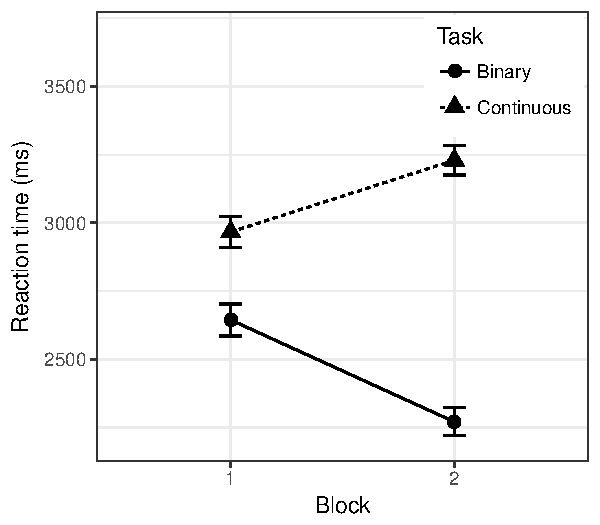
\includegraphics{images/RTorderEffects.pdf}
	\caption{Mean reaction times. Error bars are within-subject difference-adjusted confidence intervals \protect\cite{Baguley2012}.}
	\label{figure:RTblockGraph}
\end{figure}


% Table created by stargazer v.5.2.2 by Marek Hlavac, Harvard University. E-mail: hlavac at fas.harvard.edu
% Date and time: Tue, Jun 04, 2019 - 15:10:04
\begin{table}[t] \centering 
  \caption{Summary of coefficients of model predicting reaction time} 
  \label{table:rtModel} 
\begin{tabular}{@{\extracolsep{5pt}}lc} 
\\[-1.8ex]\hline 
\hline \\[-1.8ex] 
 & \multicolumn{1}{c}{\textit{Dependent variable:}} \\ 
\cline{2-2} 
\\[-1.8ex] & rt \\ 
\hline \\[-1.8ex] 
 Task & 299.238 ($-$313.417, 911.894) \\ 
  $\vert\Delta_A\vert$ & $-$801.637$^{**}$ ($-$1,415.806, $-$187.468) \\ 
  $\vert\Delta_V\vert$ & $-$90.223$^{**}$ ($-$175.690, $-$4.757) \\ 
  Task : $\vert\Delta_A\vert$ & $-$143.654 ($-$977.778, 690.469) \\ 
  Task : $\vert\Delta_V\vert$ & 11.538 ($-$103.462, 126.537) \\ 
  $\vert\Delta_A\vert$ : $\vert\Delta_V\vert$ & 12.598 ($-$282.011, 307.207) \\ 
  Task : $\vert\Delta_A\vert$ :  $\vert\Delta_V\vert$ & 120.222 ($-$274.293, 514.737) \\ 
  Constant & 2,989.224$^{***}$ (2,547.009, 3,431.439) \\ 
 \hline \\[-1.8ex] 
Observations & 2,557 \\ 
Log Likelihood & $-$21,556.920 \\ 
Akaike Inf. Crit. & 43,135.830 \\ 
Bayesian Inf. Crit. & 43,200.140 \\ 
\hline 
\hline \\[-1.8ex] 
\textit{Note:}  & \multicolumn{1}{l}{\footnotesize $\vert\Delta_A\vert$ = absolute attention difference; $\vert\Delta_V\vert$ = absolute value difference; } \\ 
\end{tabular} 
\end{table} 


There was a significant variance in reaction time intercepts across participants, $SD=1114.18$ (95\% CI: 900.45, 1378.63), $\chi^2(1)=1375.60$, $p<.001$. Additionally, slopes based on absolute difference in attention ($|\Delta_A|$) significantly varied across participants, $SD=556.09$ (95\% CI: 275.62, 1121.96), $\chi(1)=8.21$, $p=.004$. As did the slopes based on absolute difference in value ($|\Delta_V|$), $SD=90.54$ (95\% CI: 52.81, 155.24), $\chi(1)=8.34$, $p=.004$. Therefore, the final model included main effects of task, attention and value, with random effects of attention and value. 

\begin{figure}[b!]
	\centering
	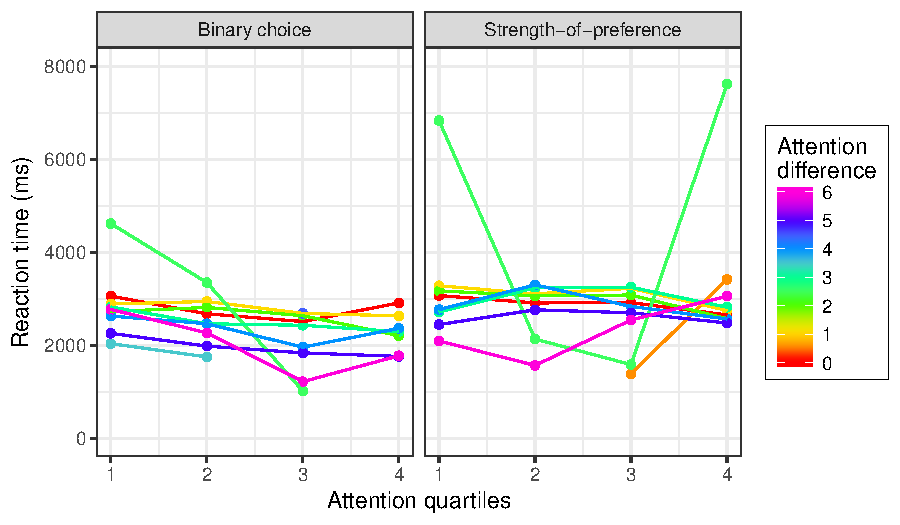
\includegraphics{images/RTattentionValueGraph}
	\caption{Looking at reaction time across difference in attention quartiles, where 1=not much difference in attention between options, 4 a lot of difference in attention between options.}
	\label{figure:RTattentionValueGraph}
\end{figure}

\begin{figure}[b!]
	\centering
	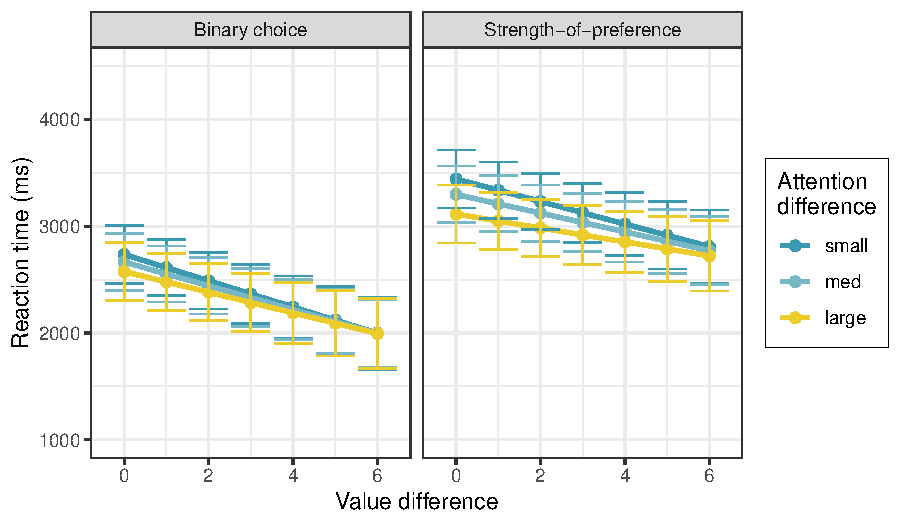
\includegraphics{images/predictedRTattentionValueGraph.pdf}
	\caption{Predicted reaction times based on the model.}
	\label{figure:predictedRTattentionValueGraph}
\end{figure}

Table~\ref{table:rtModel} contains the coefficients and 95\% confidence intervals for the fixed effects in the full reaction time model (see Figure~\ref{figure:RTattentionValueGraph}). In summary, reaction times were significantly predicted by difference in attention, $t=2.44$, $SE=318.49$, $p=.015$. The greater the difference in amount of attention between the two options, the faster the participant responded. There was also an effect of difference in value, $t=2.03$, $SE=43.70$, $p=.043$. The greater the difference in value between the choices, the faster participants responded. The main effect of task, the two-way and three-way interactions did not reach significance ($p>=0.331$). 

\subsection{Choice}
To consider a mixed effects model of choice, we recoded the responses given in the continuous task as binary. Other ways of completing this analysis, which attempted to take into account the additional information available in the continuous tasks (such as linear probability models), found similar results. 

There was no interaction between task and order on choice, $p=.766$. Additionally, a main effects analysis found the four-way interaction was not significant, $p=.999$. However, there was a significant effect of task order on reaction time, so here we report an analysis of the first block only. 

There was a significant random effect of difference in attention on choice, $\chi^2(1)=1791.02$, $p<.001$. There was also a random effect of difference in value on choice, $\chi^2(1)=1341.70$, $p<.001$. A random effect of task did not add additional information, $\chi^2(3)=0.46$, $p=.928$. Therefore, the final model included fixed effects of task, attention and value, with random effects of attention and value.

Table~\ref{table:choiceModelBlock1} contains the coefficients and 95\% confidence intervals for the fixed effects in the full choice model for the first block only (the preregistered analysis). Choice was significantly predicted by attention, $t(1)=12.89$, $SE=0.44$, $p<.001$, and value, $t(1)=14.28$, $SE=0.06$, $p<.001$. In other words, the picture that was looked at more was more likely to be picked, as was the picture that the participant preferred. The main effect of task, as well as two- and three-way interactions did not reach significance ($p>=.168$). The predicted choice probabilities are shown in Figure~\ref{figure:predictedChoiceGraph}.


% Table created by stargazer v.5.2.2 by Marek Hlavac, Harvard University. E-mail: hlavac at fas.harvard.edu
% Date and time: Wed, Nov 20, 2019 - 12:21:11
\begin{table}[!b] \centering 
  \caption{Summary of coefficients of model predicting choice (both blocks).} 
  \label{table:choiceModelAll} 
\begin{tabular}{@{\extracolsep{5pt}}lc} 
\\[-1.8ex]\hline 
\hline \\[-1.8ex] 
 & \multicolumn{1}{c}{\textit{Dependent variable:}} \\ 
\cline{2-2} 
\\[-1.8ex] & recodedResponse \\ 
\hline \\[-1.8ex] 
 Task & $-$2.070 ($-$5.292, 1.153) \\ 
  $\Delta_A$ & $-$9.063$^{***}$ ($-$13.782, $-$4.345) \\ 
  $\Delta_V$ & $-$0.908$^{***}$ ($-$1.227, $-$0.589) \\ 
  Task : $\Delta_A$ & $-$0.021 ($-$0.542, 0.500) \\ 
  Task : $\Delta_V$ & 4.059 ($-$2.355, 10.474) \\ 
  $\Delta_A$ : $\Delta_V$ & 0.300 ($-$0.129, 0.728) \\ 
  Task : $\Delta_A$ :  $\Delta_V$ & $-$0.328 ($-$1.038, 0.382) \\ 
  Constant & 4.598$^{***}$ (2.231, 6.965) \\ 
 \hline \\[-1.8ex] 
Observations & 2,557 \\ 
Log Likelihood & $-$956.750 \\ 
Akaike Inf. Crit. & 1,933.499 \\ 
Bayesian Inf. Crit. & 1,991.965 \\ 
\hline 
\hline \\[-1.8ex] 
\textit{Note:}  & \multicolumn{1}{l}{\footnotesize $\Delta_A$ = attention difference; $\Delta_V$ = value difference; } \\ 
\end{tabular} 
\end{table} 


% Table created by stargazer v.5.2.2 by Marek Hlavac, Harvard University. E-mail: hlavac at fas.harvard.edu
% Date and time: Wed, Jun 26, 2019 - 10:53:55
\begin{table}[!b] \centering 
  \caption{Summary of coefficients of model predicting choice (Block 1 only).} 
  \label{table:choiceModelBlock1} 
\begin{tabular}{@{\extracolsep{5pt}}lc} 
\\[-1.8ex]\hline 
\hline \\[-1.8ex] 
 & \multicolumn{1}{c}{\textit{Dependent variable:}} \\ 
\cline{2-2} 
\\[-1.8ex] & recodedResponse \\ 
\hline \\[-1.8ex] 
 Task & $-$0.073 ($-$0.383, 0.237) \\ 
  $\Delta_A$ & 6.556$^{***}$ (5.137, 7.976) \\ 
  $\Delta_V$ & 0.933$^{***}$ (0.746, 1.119) \\ 
  Task : $\Delta_A$ & 0.127 ($-$1.812, 2.067) \\ 
  Task : $\Delta_V$ & $-$0.129 ($-$0.373, 0.114) \\ 
  $\Delta_A$ : $\Delta_V$ & 0.025 ($-$0.555, 0.604) \\ 
  Task : $\Delta_A$ :  $\Delta_V$ & $-$0.025 ($-$0.795, 0.746) \\ 
  Constant & 0.068 ($-$0.157, 0.293) \\ 
 \hline \\[-1.8ex] 
Observations & 2,557 \\ 
Log Likelihood & $-$931.833 \\ 
Akaike Inf. Crit. & 1,885.665 \\ 
Bayesian Inf. Crit. & 1,949.978 \\ 
\hline 
\hline \\[-1.8ex] 
\textit{Note:}  & \multicolumn{1}{l}{\footnotesize $\Delta_A$ = attention difference; $\Delta_V$ = value difference; } \\ 
\end{tabular} 
\end{table} 


% Table created by stargazer v.5.2.2 by Marek Hlavac, Harvard University. E-mail: hlavac at fas.harvard.edu
% Date and time: Wed, Jun 26, 2019 - 10:54:04
\begin{table}[!b] \centering 
  \caption{Summary of coefficients of model predicting choice (Block 2 only).} 
  \label{table:choiceModelBlock2} 
\begin{tabular}{@{\extracolsep{5pt}}lc} 
\\[-1.8ex]\hline 
\hline \\[-1.8ex] 
 & \multicolumn{1}{c}{\textit{Dependent variable:}} \\ 
\cline{2-2} 
\\[-1.8ex] & recodedResponse \\ 
\hline \\[-1.8ex] 
 Task & $-$0.004 ($-$0.259, 0.252) \\ 
  $\Delta_A$ & 5.199$^{***}$ (3.984, 6.414) \\ 
  $\Delta_V$ & 0.909$^{***}$ (0.727, 1.090) \\ 
  Task : $\Delta_A$ & 0.974 ($-$0.809, 2.758) \\ 
  Task : $\Delta_V$ & 0.106 ($-$0.154, 0.365) \\ 
  $\Delta_A$ : $\Delta_V$ & 0.071 ($-$0.368, 0.509) \\ 
  Task : $\Delta_A$ :  $\Delta_V$ & $-$0.195 ($-$0.951, 0.561) \\ 
  Constant & $-$0.017 ($-$0.190, 0.156) \\ 
 \hline \\[-1.8ex] 
Observations & 2,558 \\ 
Log Likelihood & $-$961.365 \\ 
Akaike Inf. Crit. & 1,944.730 \\ 
Bayesian Inf. Crit. & 2,009.047 \\ 
\hline 
\hline \\[-1.8ex] 
\textit{Note:}  & \multicolumn{1}{l}{\footnotesize $\Delta_A$ = attention difference; $\Delta_V$ = value difference;} \\ 
\end{tabular} 
\end{table} 


\begin{figure}
	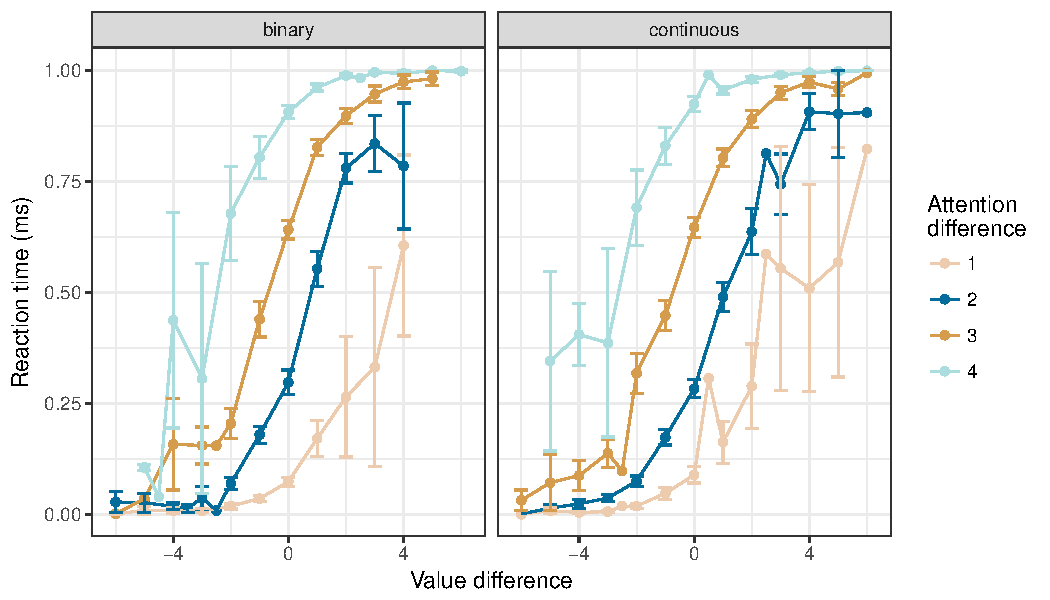
\includegraphics{images/predictedChoiceGraph}
	\caption{Predicted choice probabilities from the model, based on the first block only.}
	\label{figure:predictedChoiceGraph}	
\end{figure}


Also included are the outputs for both blocks together (Table~\ref{table:choiceModelAll}) and for the final block on its own (Table~\ref{table:choiceModelBlock2}). The final block version is perhaps interesting as the reaction time analyses showed that the difference in reaction was greater for the second block than the first. Although this did change the coefficients slightly, the confidence intervals are still securely including 0. 

\subsection{Distribution of continuous responses}
In Figure~\ref{figure:continuousResponses} are reported the distributions of responses given by participants. 

\begin{figure}[!b]
	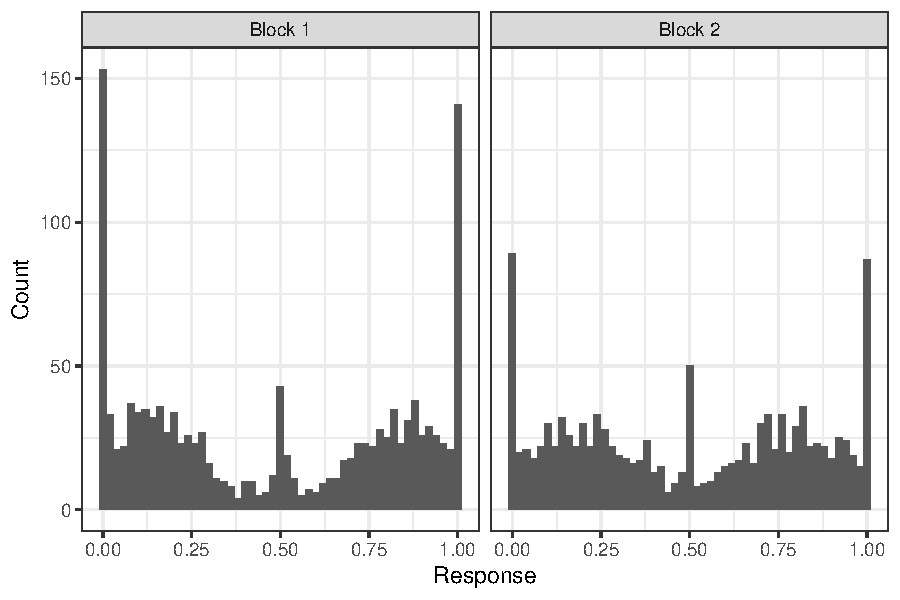
\includegraphics{images/continuousResponses}
	\caption{Histogram of the responses given by participants in the continuous task, separated by task order.}
	\label{figure:continuousResponses}
\end{figure}

\clearpage
\newpage
\section{Alternative analyses}
In the following we look to see if the \emph{pattern} of attention is different between these two tasks. 

\subsection{Number of fixations}
Here, we operationalized ``number of fixations'' as 
\begin{equation}
	\frac{N_\text{right}}{N_\text{left}+N_\text{right}}
\end{equation}
where $N_i$ is the number of fixation on option $i$. 

There was significant variance of participant on proportion of number of fixations, $\chi^2(1)=25.97$, $p<.001$. Therefore, the model included fixed effects of task, attention and value with their interactions and a random effect of participant on the intercepts. As shown in Table~\ref{table:nFixModel}, nothing really came out. 


% Table created by stargazer v.5.2.2 by Marek Hlavac, Harvard University. E-mail: hlavac at fas.harvard.edu
% Date and time: Tue, Jun 04, 2019 - 15:10:30
\begin{table}[!b] \centering 
  \caption{Summary of coefficients of model predicting number of fixations on each choice} 
  \label{table:nFixModel} 
\begin{tabular}{@{\extracolsep{5pt}}lc} 
\\[-1.8ex]\hline 
\hline \\[-1.8ex] 
 & \multicolumn{1}{c}{\textit{Dependent variable:}} \\ 
\cline{2-2} 
\\[-1.8ex] & relativeFixN \\ 
\hline \\[-1.8ex] 
 Task & $-$0.013 ($-$0.042, 0.015) \\ 
  $\Delta_A$ & $-$0.012 ($-$0.079, 0.054) \\ 
  $\Delta_V$ & 0.007 ($-$0.002, 0.015) \\ 
  Task : $\Delta_A$ & 0.013 ($-$0.073, 0.098) \\ 
  Task : $\Delta_V$ & $-$0.003 ($-$0.013, 0.008) \\ 
  $\Delta_A$ : $\Delta_V$ & 0.00005 ($-$0.031, 0.031) \\ 
  Task : $\Delta_A$ :  $\Delta_V$ & 0.022 ($-$0.018, 0.061) \\ 
  Constant & 0.467$^{***}$ (0.445, 0.489) \\ 
 \hline \\[-1.8ex] 
Observations & 1,009 \\ 
Log Likelihood & 311.125 \\ 
Akaike Inf. Crit. & $-$602.250 \\ 
Bayesian Inf. Crit. & $-$553.083 \\ 
\hline 
\hline \\[-1.8ex] 
\textit{Note:}  & \multicolumn{1}{l}{\footnotesize $\Delta_A$ = attention difference; $\Delta_V$ = value difference; } \\ 
\end{tabular} 
\end{table} 




\clearpage
\subsection{Duration of fixations}
Here, duration of fixations was operationalized as 
\begin{equation}
	\frac{D_{right}}{D_{left} + D_{right}}
\end{equation}
where $D_i$ was the mean duration of fixations on option $i$. 

Including random effects did not improve the explanatory power of this model. Further, as seen in Table~\ref{table:durFixModel}, nothing came out. 


% Table created by stargazer v.5.2.2 by Marek Hlavac, Harvard University. E-mail: hlavac at fas.harvard.edu
% Date and time: Tue, Jun 18, 2019 - 17:55:33
\begin{table}[!b] \centering 
  \caption{Summary of coefficients of model predicting duration of time on options} 
  \label{table:durFixModel} 
\begin{tabular}{@{\extracolsep{5pt}}lc} 
\\[-1.8ex]\hline 
\hline \\[-1.8ex] 
 & \multicolumn{1}{c}{\textit{Dependent variable:}} \\ 
\cline{2-2} 
\\[-1.8ex] & relativeFixDur \\ 
\hline \\[-1.8ex] 
 Task & $-$0.0005 ($-$0.005, 0.004) \\ 
  $\Delta_A$ & 0.001$^{***}$ (0.001, 0.001) \\ 
  $\Delta_V$ & 0.002$^{**}$ (0.0003, 0.003) \\ 
  Task : $\Delta_A$ & 0.0001$^{***}$ (0.00004, 0.0001) \\ 
  Task : $\Delta_V$ & $-$0.00005 ($-$0.002, 0.002) \\ 
  $\Delta_A$ : $\Delta_V$ & $-$0.00001$^{*}$ ($-$0.00002, 0.00000) \\ 
  Task : $\Delta_A$ :  $\Delta_V$ & $-$0.00000 ($-$0.00001, 0.00001) \\ 
  Constant & 0.503$^{***}$ (0.500, 0.506) \\ 
 \hline \\[-1.8ex] 
Observations & 2,509 \\ 
Log Likelihood & 4,197.527 \\ 
Akaike Inf. Crit. & $-$8,375.054 \\ 
Bayesian Inf. Crit. & $-$8,316.778 \\ 
\hline 
\hline \\[-1.8ex] 
\textit{Note:}  & \multicolumn{1}{l}{\footnotesize $\Delta_A$ = attention difference; $\Delta_V$ = value difference; } \\ 
\end{tabular} 
\end{table} 


\clearpage
\newpage
\subsection{Looking at different ways of operationalizing attention}
In the above analyses, attention was operationalized as 

\begin{equation}
	\frac{T_{right}-T_{left}}{RT}	
\end{equation}
where $T_i$ is the total time spent fixating on option $i$ and $RT$ is the reaction time. 

However, previously Tim has used

\begin{equation}
	\frac{T_{right}-T_{left}}{T_{right}+T_{left}}
\end{equation}
where attention is normalized out of the total time spent looking at options. 

Also, CERE noticed that participants appear to spend more time looking at the Likert scale in the strength-of-preference task than in the binary task. Especially when the participants appeared to be undecided between the two options. Therefore, 

\begin{equation}
	\frac{T_\text{right}-T_\text{left}}{T_\text{right}+T_\text{left}+T_\text{likert}}
\end{equation}
is a measure of difference of attention normalised by time spent on task. 

% Table created by stargazer v.5.2.2 by Marek Hlavac, Harvard University. E-mail: hlavac at fas.harvard.edu
% Date and time: Tue, Jun 04, 2019 - 15:26:42
\begin{table}[h] \centering 
  \caption{Summary of coefficients of model predicting choice, comparing different attentions} 
  \label{table:choiceModelAttention} 
\begin{tabular}{@{\extracolsep{5pt}}lccc} 
\\[-1.8ex]\hline 
\hline \\[-1.8ex] 
 & \multicolumn{3}{c}{\textit{Dependent variable:}} \\ 
\cline{2-4} 
\\[-1.8ex] & \multicolumn{3}{c}{recodedResponse} \\ 
 & by reaction time & by time on choices & by time on task \\ 
\\[-1.8ex] & (1) & (2) & (3)\\ 
\hline \\[-1.8ex] 
 Task & 0.014 & 0.010 & 0.012 \\ 
  & ($-$0.495, 0.523) & ($-$0.497, 0.518) & ($-$0.502, 0.527) \\ 
  & & & \\ 
 $\Delta_A$ & 5.928$^{***}$ & 4.503$^{***}$ & 4.530$^{***}$ \\ 
  & (3.520, 8.336) & (2.691, 6.315) & (2.664, 6.397) \\ 
  & & & \\ 
 $\Delta_V$ & 1.007$^{***}$ & 0.999$^{***}$ & 1.002$^{***}$ \\ 
  & (0.749, 1.266) & (0.742, 1.255) & (0.746, 1.258) \\ 
  & & & \\ 
 Task : $\Delta_A$ & 0.416 & 0.035 & 0.307 \\ 
  & ($-$2.710, 3.541) & ($-$2.296, 2.366) & ($-$2.114, 2.728) \\ 
  & & & \\ 
 Task : $\Delta_V$ & $-$0.268$^{*}$ & $-$0.258 & $-$0.257 \\ 
  & ($-$0.583, 0.047) & ($-$0.571, 0.056) & ($-$0.569, 0.056) \\ 
  & & & \\ 
 $\Delta_A$ : $\Delta_V$ & $-$0.270 & $-$0.195 & $-$0.200 \\ 
  & ($-$1.320, 0.781) & ($-$0.997, 0.606) & ($-$1.005, 0.605) \\ 
  & & & \\ 
 Task : $\Delta_A$ :  $\Delta_V$ & 0.571 & 0.402 & 0.416 \\ 
  & ($-$0.693, 1.834) & ($-$0.545, 1.350) & ($-$0.544, 1.376) \\ 
  & & & \\ 
 Constant & $-$0.129 & $-$0.123 & $-$0.123 \\ 
  & ($-$0.523, 0.265) & ($-$0.516, 0.270) & ($-$0.520, 0.275) \\ 
  & & & \\ 
\hline \\[-1.8ex] 
Observations & 1,009 & 1,009 & 1,009 \\ 
Log Likelihood & $-$376.774 & $-$379.472 & $-$376.175 \\ 
Akaike Inf. Crit. & 775.547 & 780.945 & 774.351 \\ 
Bayesian Inf. Crit. & 829.631 & 835.029 & 828.435 \\ 
\hline 
\hline \\[-1.8ex] 
\textit{Note:}  & \multicolumn{3}{l}{\footnotesize $\Delta_A$ = attention difference; $\Delta_V$ = value difference; } \\ 
\end{tabular} 
\end{table} 



% Table created by stargazer v.5.2.2 by Marek Hlavac, Harvard University. E-mail: hlavac at fas.harvard.edu
% Date and time: Mon, Jun 17, 2019 - 11:22:41
\begin{table}[h] \centering 
  \caption{Summary of coefficients of model predicting reaction time, comparing different attentions} 
  \label{table:choiceModelAttention} 
\begin{tabular}{@{\extracolsep{5pt}}lccc} 
\\[-1.8ex]\hline 
\hline \\[-1.8ex] 
 & \multicolumn{3}{c}{\textit{Dependent variable:}} \\ 
\cline{2-4} 
\\[-1.8ex] & \multicolumn{3}{c}{rt} \\ 
 & by reaction time & by time on choices & by time on task \\ 
\\[-1.8ex] & (1) & (2) & (3)\\ 
\hline \\[-1.8ex] 
 Task & 299.238 & 279.020 & 283.355 \\ 
  & ($-$313.417, 911.894) & ($-$331.747, 889.786) & ($-$325.781, 892.491) \\ 
  & & & \\ 
 $\vert\Delta_A\vert$ & $-$801.637$^{**}$ & $-$742.610$^{***}$ & $-$781.693$^{***}$ \\ 
  & ($-$1,415.806, $-$187.468) & ($-$1,202.525, $-$282.694) & ($-$1,242.441, $-$320.945) \\ 
  & & & \\ 
 $\vert\Delta_V\vert$ & $-$90.223$^{**}$ & $-$94.532$^{**}$ & $-$96.018$^{**}$ \\ 
  & ($-$175.690, $-$4.757) & ($-$179.640, $-$9.425) & ($-$181.018, $-$11.019) \\ 
  & & & \\ 
 Task : $\vert\Delta_A\vert$ & $-$143.654 & $-$3.025 & $-$33.773 \\ 
  & ($-$977.778, 690.469) & ($-$628.369, 622.319) & ($-$660.869, 593.322) \\ 
  & & & \\ 
 Task : $\vert\Delta_V\vert$ & 11.538 & 10.815 & 17.079 \\ 
  & ($-$103.462, 126.537) & ($-$104.698, 126.327) & ($-$97.826, 131.984) \\ 
  & & & \\ 
 $\vert\Delta_A\vert$ : $\vert\Delta_V\vert$ & 12.598 & 29.257 & 34.950 \\ 
  & ($-$282.011, 307.207) & ($-$192.471, 250.985) & ($-$187.217, 257.118) \\ 
  & & & \\ 
 Task : $\vert\Delta_A\vert$ :  $\vert\Delta_V\vert$ & 120.222 & 86.562 & 69.510 \\ 
  & ($-$274.293, 514.737) & ($-$205.962, 379.085) & ($-$224.469, 363.488) \\ 
  & & & \\ 
 Constant & 2,989.224$^{***}$ & 3,028.362$^{***}$ & 3,038.606$^{***}$ \\ 
  & (2,547.009, 3,431.439) & (2,588.554, 3,468.171) & (2,599.546, 3,477.667) \\ 
  & & & \\ 
\hline \\[-1.8ex] 
Observations & 2,557 & 2,557 & 2,557 \\ 
Log Likelihood & $-$21,556.920 & $-$21,554.310 & $-$21,551.030 \\ 
Akaike Inf. Crit. & 43,135.830 & 43,130.620 & 43,124.060 \\ 
Bayesian Inf. Crit. & 43,200.140 & 43,194.930 & 43,188.370 \\ 
\hline 
\hline \\[-1.8ex] 
\textit{Note:}  & \multicolumn{3}{l}{\footnotesize $\vert\Delta_A\vert$ = absolute attention difference; $\vert\Delta_V\vert$ = absolute value difference; } \\ 
\end{tabular} 
\end{table} 


Mainly because (as shown in Figure~\ref{figure:attentionCorrelations}) they all correlate pretty perfectly. 

\begin{figure}
	\centering
	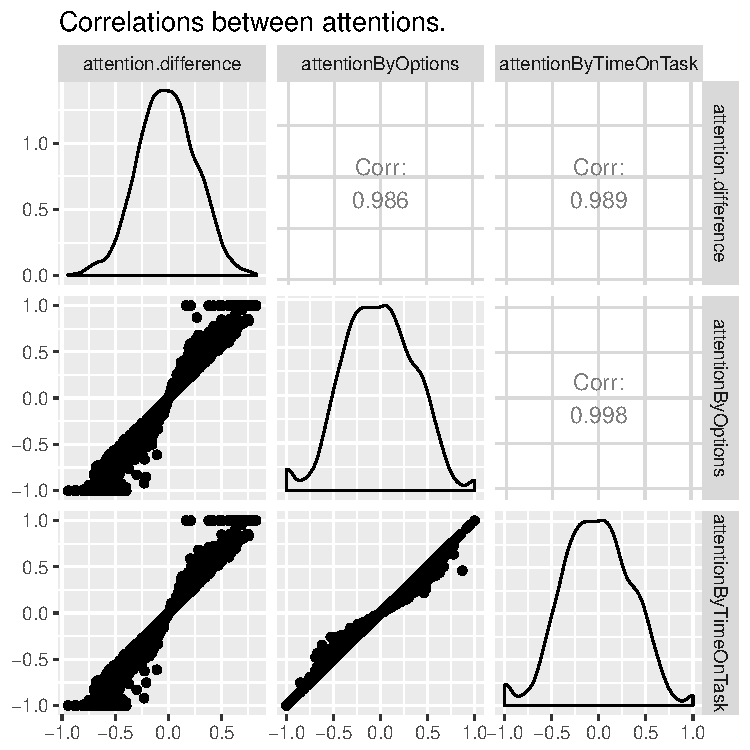
\includegraphics[width=0.7\textwidth]{images/attentionCorrelations}
	\caption{Correlations between different metrics of attention}
	\label{figure:attentionCorrelations}
\end{figure}

\clearpage
\section{Overall value}

\citeA{Smith:2018iz} looked at overall value along with value difference to predict reaction time using the model:

\begin{equation}
	\log(RT) \sim \beta_0 + \beta_1|V_\text{left} - V_\text{right}| + \beta_2(V_\text{left} + V_\text{right})
\end{equation}
where $V_i$ is the subjective value of option $i$. I do a similar thing below. Using this model, we fail to replicate their findings. In this experiment, there is a main effect of absolute difference in value ($\Delta_V$), $\beta_1=-75.24$, $t=3.53$, $SE=21.32$, $p<.001$. In other words, the greater the difference in value between the choices, the faster participants were. However, there is no main effect of total value, $\beta_2=11.39$, $t=0.85$, $SE=13.36$, $p=.394$.


% Table created by stargazer v.5.2.2 by Marek Hlavac, Harvard University. E-mail: hlavac at fas.harvard.edu
% Date and time: Tue, Jun 04, 2019 - 16:14:10
\begin{table}[!b] \centering 
  \caption{Summary of coefficients of model predicting reaction time from total value and value difference} 
  \label{table:rtModelSmithTask} 
\begin{tabular}{@{\extracolsep{5pt}}lc} 
\\[-1.8ex]\hline 
\hline \\[-1.8ex] 
 & \multicolumn{1}{c}{\textit{Dependent variable:}} \\ 
\cline{2-2} 
\\[-1.8ex] & rt \\ 
\hline \\[-1.8ex] 
 Task & 720.525$^{**}$ (14.210, 1,426.840) \\ 
  $\sum_A$ & 41.222 ($-$13.101, 95.545) \\ 
  $\Delta_V$ & $-$90.698 ($-$379.134, 197.737) \\ 
  Task : $\sum_A$ & $-$60.676 ($-$138.112, 16.760) \\ 
  Task : $\Delta_V$ & 60.638 ($-$341.784, 463.060) \\ 
  $\sum_A$ : $\Delta_V$ & $-$3.902 ($-$37.350, 29.547) \\ 
  Task : $\sum_A$ :  $\Delta_V$ & 2.386 ($-$44.019, 48.790) \\ 
  Constant & 2,490.447$^{***}$ (2,001.486, 2,979.407) \\ 
 \hline \\[-1.8ex] 
Observations & 2,557 \\ 
R$^{2}$ & 0.021 \\ 
Adjusted R$^{2}$ & 0.018 \\ 
Residual Std. Error & 1,479.557 (df = 2549) \\ 
F Statistic & 7.728$^{***}$ (df = 7; 2549) \\ 
\hline 
\hline \\[-1.8ex] 
\textit{Note:}  & \multicolumn{1}{l}{\footnotesize $\sum_A$ = total value; $\Delta_V$ = value difference; } \\ 
\end{tabular} 
\end{table} 


Of course, using this model is silly because this collapses across tasks. Therefore, we also ran a linear model that looked at $\Delta_V$, total value and task on reaction time in the first block (see Table~\ref{table:rtModelSmithTask}). Here, we just found a main effect of task, $t=2.00$, $SE=360.37$, $p=.046$.


\clearpage
\section{Open Practices Statement}
The analysis was pre-registered at \url{AsPredicted.org/19698}. The data and analysis of this experiment is available in the Open Science Framework \url{https://osf.io/xfc8a/}. 




\clearpage
\section{Appendix}
\subsection{Choice model including all trials}
Here, we consider the model of choice including all trials (i.e. no exclusions based on reaction time) for the first block. The model for the second block is similar. 

There was a significant random effect of difference in attention on choice, $\chi^2(1)=985.41$, $p<.001$. There was also a random effect of difference in value on choice, $\chi^2(1)=569.79$, $p<.001$. A random effect of task did not add additional information, $\chi^2(3)=0.02$, $p=.999$. Therefore, the final model included fixed effects of task, attention and value, with random effects of attention and value.


% Table created by stargazer v.5.2.2 by Marek Hlavac, Harvard University. E-mail: hlavac at fas.harvard.edu
% Date and time: Tue, Jun 04, 2019 - 15:38:55
\begin{table}[!b] \centering 
  \caption{Summary of coefficients of model predicting choice including all trials} 
  \label{table:choiceModelAllTrials} 
\begin{tabular}{@{\extracolsep{5pt}}lc} 
\\[-1.8ex]\hline 
\hline \\[-1.8ex] 
 & \multicolumn{1}{c}{\textit{Dependent variable:}} \\ 
\cline{2-2} 
\\[-1.8ex] & recodedResponse \\ 
\hline \\[-1.8ex] 
 Task & $-$0.083 ($-$0.382, 0.216) \\ 
  $\Delta_A$ & 6.436$^{***}$ (5.019, 7.853) \\ 
  $\Delta_V$ & 0.926$^{***}$ (0.740, 1.113) \\ 
  Task : $\Delta_A$ & 0.446 ($-$1.486, 2.379) \\ 
  Task : $\Delta_V$ & $-$0.146 ($-$0.388, 0.096) \\ 
  $\Delta_A$ : $\Delta_V$ & 0.059 ($-$0.513, 0.631) \\ 
  Task : $\Delta_A$ :  $\Delta_V$ & $-$0.039 ($-$0.793, 0.714) \\ 
  Constant & 0.061 ($-$0.157, 0.280) \\ 
 \hline \\[-1.8ex] 
Observations & 2,650 \\ 
Log Likelihood & $-$969.822 \\ 
Akaike Inf. Crit. & 1,961.644 \\ 
Bayesian Inf. Crit. & 2,026.349 \\ 
\hline 
\hline \\[-1.8ex] 
\textit{Note:}  & \multicolumn{1}{l}{\footnotesize $\Delta_A$ = attention difference; $\Delta_V$ = value difference; } \\ 
\end{tabular} 
\end{table} 


Table~\ref{table:choiceModel} contains the coefficients and 95\% confidence intervals for the fixed effects in the full choice model. Choice was significantly predicted by attention, $t(1)=8.90$, $SE=0.72$, $p<.001$, and value, $t(1)=9.73$, $SE=0.10$, $p<.001$. In other words, the picture that was looked at more was more likely to be picked, as was the picture that the participant preferred. The main effect of task, as well as two- and three-way interactions did not reach significance ($p>=.237$).



\clearpage
\newpage
\bibliographystyle{apacite}
\bibliography{references}

\end{document}